 \chapter{Overview of Concepts} 
 
 %Research projects should always be based on previous research on the same and/or related topics. This should be described as a background to the thesis with adequate bibliographical references. If the material needed is too voluminous to fit nicely in the review part of the introduction, it can be presented in a separate background chapter.
In order to get a theoretical overview of topics related to the detection and mitigation of \acrlong{tsa} attacks targeting \acrlong{sg}s, the concept of \acrfull{sg} is explained, as well as aspects related to the \acrshort{sg} architecture, and \acrshort{sg} vulnerabilities. 


Before studying the \acrshort{sg} in more detail,  some introductory terms are covered.  



\section{Critical (Information) Infrastructure}

The term Critical Infrastructure, denotes infrastructure critical to the operation of some function, or service, vital to its recipients. As a result of the society being more dependant on the availability of electronic services, the flow of electricity from the \acrshort{pg} \acrfull{ci} is dependant on networking provided by \acrfull{cii}.\\ 

\textbf{\acrfull{ci}} is, in  \cite{luiijf2012understanding}, defined as ... 
 \begin{quote}
"... an asset, system or part thereof located in a
nation which is essential for the maintenance of vital societal functions, health, safety,
security, economic or social well-being of people, and the disruption or destruction of
which would have a significant impact in that nation as a result of the failure to maintain
those functions." \cite[p. 53]{luiijf2012understanding}     
 \end{quote}
 

\textbf{\acrfull{cii}} is, in  \cite{luiijf2012understanding}, defined as ...
 \begin{quote}
" ... those interconnected information
systems and networks, the disruption or destruction of which would have a
serious impact on the health, safety, security, or economic well-being of citizens, or
on the effective functioning of government or the economy." \cite[p. 53]{luiijf2012understanding}     
 \end{quote}


The \acrshort{cii} is fundamental to the proper operation of the \acrshort{ci}, and is dependant on the availaibility of \acrfull{ict} and \acrfull{telco} \acrlong{ci}, as 
indicated by figure \ref{fig:CI-CIII}


\begin{figure}[ht]
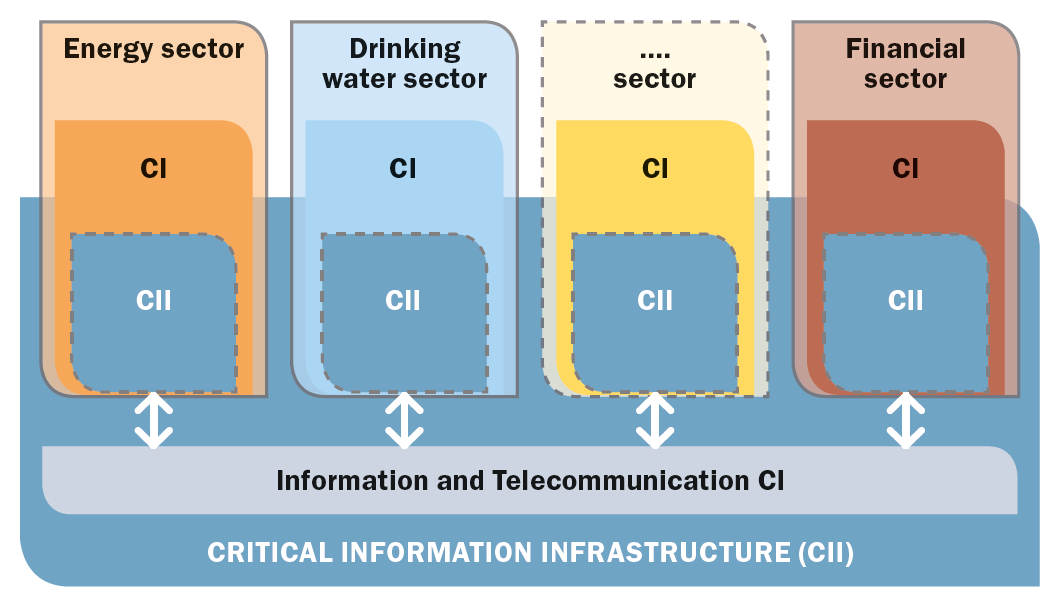
\includegraphics[width=\linewidth]{figures/CI-CII.png}
\caption[CI/CIII in the ICT and TELCO sectors]{Sector CI and CII dependency on ICT and TELCO CI. \cite{luiijf2016gfce}}
\label{fig:CI-CIII}
\end{figure}


\subsection{Critical (Information) Infrastructure Protection}

As presented in figure \ref{fig:CI-CIII}, \acrfull{ci} depends on \acrfull{cii}, as \acrshort{cii} is required in order for a distributed \acrshort{ci} like the \acrshort{sg} to operate as required. Figure \ref{fig:CI-CIII-Security} shows the relationship between Critical Infrastructure Protection and Critical Information Infrastructure Protection, as the cyber security strategies related to \acrshort{ci} protection.


\begin{figure}[ht]
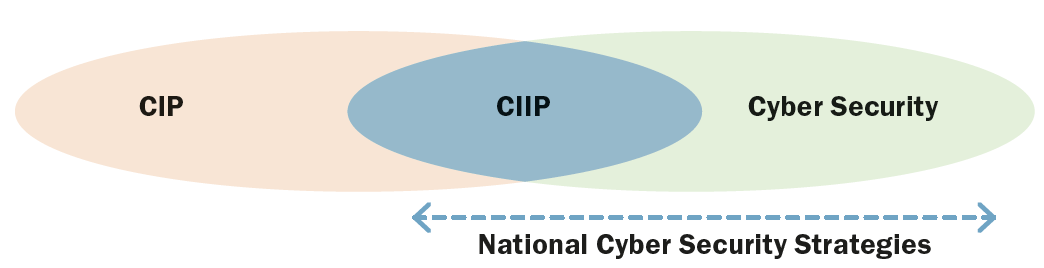
\includegraphics[width=\linewidth]{figures/CIP-CIIP-Security.png}
\caption[CIP-CIIP relations]{Relationship between Critical Infrastructure Protection and Critical Information Infrastructure Protection. \cite{luiijf2016gfce}}
\label{fig:CI-CIII-Security}
\end{figure}

\section{Cyber-Physical System}

As described by \citeauthor{humayed2017cyber} in \cite{humayed2017cyber}, a \acrfull{cps} is characterised by using a computer-based system in order to control and monitor systems of the physical world. The \acrshort{cps} is utilised in order to control physical systems from various fields of applications. Humayed et. al., in \cite{humayed2017cyber}, describes as various appliances as \acrfull{ics}, Medical Devices, and \acrlong{sg}.
The Smart Grid, therefore, is an example of a \acrfull{cps}, consisting of the physical system of a Power Grid, under the control of a network/Cyberspace-connected system. 
The \acrshort{sg} is, as described by several papers, like \cite{humayed2017cyber} and \cite{alcaraz2012security}, under the control of a \acrfull{scada} system.



\section{The Classic Power Grid }
The classic power grid is described in several papers as  a uni-directional, manually controlled, power distribution system.  

\begin{figure}[ht]
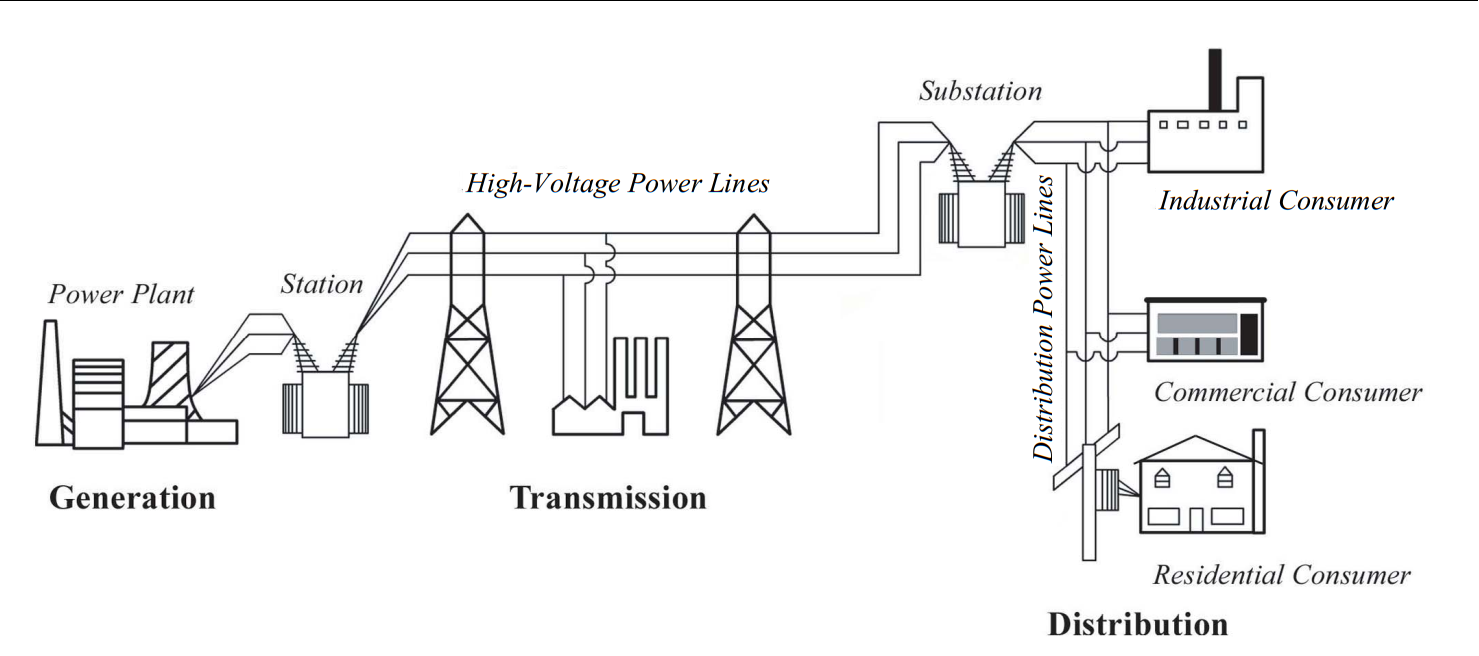
\includegraphics[width=\linewidth]{figures/Blume-PowerGrid-SystemOverView.png}
\caption[Power Grid System Overview]{Power Grid System Overview , as presented in \cite{BlumeStevenW2007Epsb}}
\label{fig:Blume-PowerGrid-SystemOverView}
\end{figure}



\subsection{Overview of the Classic Power Grid}
The Classic Power Grid is a system by which electric power is centrally generated, transmitted, and distributed to industrial, residential,and commercial end users, in order to ensure a reliable access to a sufficient amount of electrical energy. 

The classic Power Grid, as described in \cite{BlumeStevenW2007Epsb}, consists of the following subsystems:

\begin{itemize}

 \item The \textbf{Generation Subsystem} which Generates electric power from various sources of energy, to be transmitted for distribution to Consumers. Some examples of installations generating electrical power are nuclear power plants, as well as hydroelectric power plants, feeding water-driven turbines in order to generate power.
 \item The \textbf{Transmission Subsystem} which transmits electric power from the Generation subsystem to the Distribution Subsystem. The current is transmitted via high voltage power lines, minimising energy loss over longer distances.
 \item The \textbf{Distribution Subsystem} which distributes electric power to end users, after converting the high voltage input into lower voltage levels, suitable for consumption.
 \end{itemize}

As described in the introduction of \cite{SmartGridOverview2013}, the classic \acrshort{pg} is facing challenges adhering to the demands faced by a modern electricity distribution network. 


\subsection{The Classic SCADA subsystem}

The \acrshort{scada} system constituted the core part of the control center of the classic \acrlong{pg}, utilising one-directional communication lines in order to manually control and monitor the operational state of the power grid.

Figure \ref{fig:Blume-SCADA-system} shows the main components of the SCADA system.

\begin{figure}[ht]
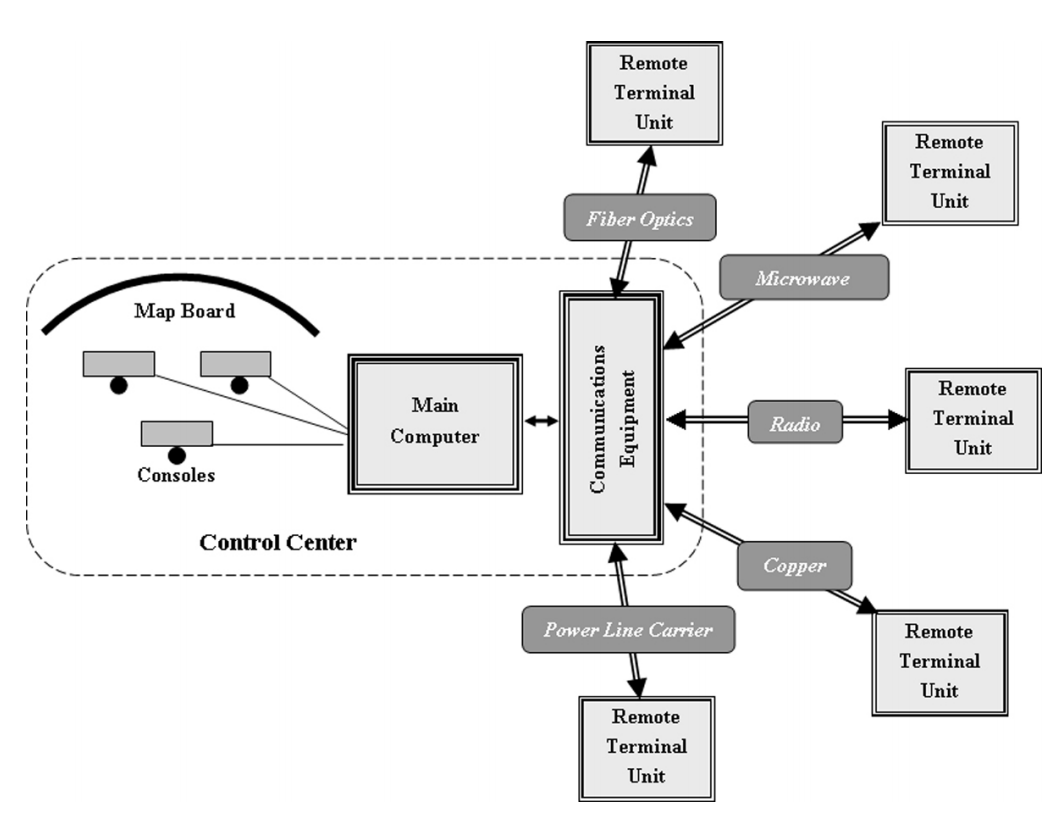
\includegraphics[width=\linewidth]{figures/Blume-SCADA-system.png}
\caption[SCADA system]{SCADA system , as presented in \cite{BlumeStevenW2007Epsb}}
\label{fig:Blume-SCADA-system}
\end{figure}

%[ \fullcite{el2008introduction} ] \\ 


A centrally located control center, optionally being backed up by control centers at one or more locations for redundancy, displays status information from the equipment at the associated substations, received for monitoring purposes. As a response to alarms indicating operational issues, commands enabling remote control of affected infrastructure is issued in order to address the issue, in order to resolve the issue and receive updated status information clearing the alarm. 









\section{The Smart Grid}




In order to provide a description of the \acrfull{sg}, a description of the characteristics of the classic \acrshort{pg} is provided.





As described in  \cite{BlumeStevenW2007Epsb} by \citeauthor{BlumeStevenW2007Epsb}, some of the characteristics of the classic power grid are:

\begin{itemize}
\item Power is generated in real time. In the event a consumer is "flipping a power switch," the power grid must have sufficient resources in order to keep the voltage levels at an acceptable level.
\item The Classic \acrlong{pg} is controlled by a central management facility known as the \acrfull{scada} subsystem. The monitoring and management of the \acrshort{pg} is initiated from the Control Center, utilising unidirectional communication channels. 
\item The Classic \acrlong{pg} \acrlong{scada} subsystem is offline, i. e. not connected to any publicly available network. Therefore, operational duties must be performed by personnel physically located at dedicated operational sites.

\end{itemize}

The classic \acrlong{pg} originates from the local society-serving power generation facilities initiating the supply of electrical power, which over the years were interconnected to form a grid, connecting consumers to a network of several power generating facilities, providing a more flexible power distribution infrastructure. 


\subsection{Overview of The Smart Grid}
The \acrshort{sg} is a part of the Critical Infrastructure of a Society, delivering a constant and reliable flow of stable and electrical power to consumers according to demand, in ways both cost efficient and friendly to the environment. The \acrshort{sg} consists of a modernised \acrshort{pg}, under the control of a network based control system. 


As described in \cite{smartgrids2012smartgrids}, the following may constitute a definition of the \acrlong{sg}:

\begin{displayquote}[{\cite[p 27]{smartgrids2012smartgrids}}]
''A SmartGrid is an electricity network that can intelligently integrate the actions of all
users connected to it - generators, consumers and those that do both – in order to
efficiently deliver sustainable, economic and secure electricity supplies.
A SmartGrid employs innovative products and services together with intelligent monitoring,
control, communication, and self-healing technologies to:
\begin{itemize}
\item better facilitate the connection and operation of generators of all sizes and technologies;
\item allow consumers to play a part in optimizing the operation of the system;
\item provide consumers with greater information and choice of supply;
\item significantly reduce the environmental impact of the whole electricity supply system;
\item deliver enhanced levels of reliability and security of supply.
\end{itemize}
SmartGrid deployment must include not only technology, market and commercial
considerations, environmental impact, regulatory framework, standardization usage, ICT
(Information \& Communication Technology) and migration strategy but also societal
requirements and governmental edicts. 
'' 
\end{displayquote}

The \acrfull{nist} has published a conceptual model of the smart grid, as shown in 
figure \ref{fig:NIST-SmartGRID-ConceptualModel}.



\begin{figure}[ht]
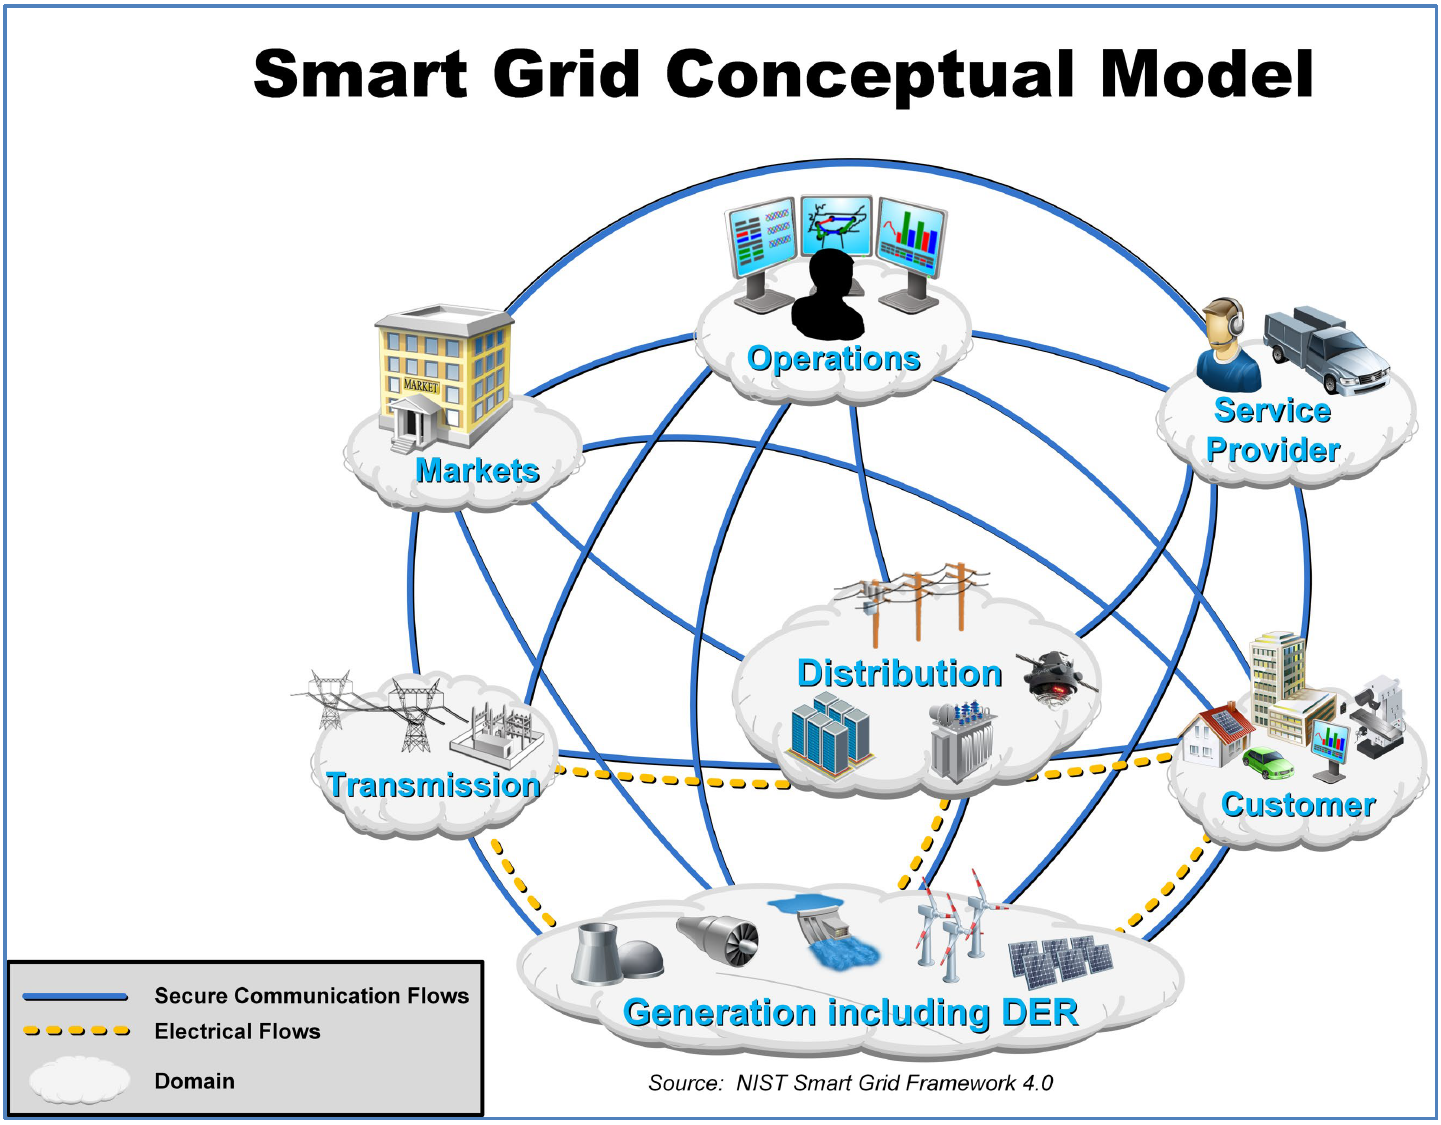
\includegraphics[width=\linewidth]{figures/NIST-SmartGRID-ConceptualModel.png}
\caption[Interactions of roles in SmartGrid Domains]{Interaction of Roles in Different \acrlong{sg} Domains through Secure Communication, as presented in \cite{greer2014nist}}
\label{fig:NIST-SmartGRID-ConceptualModel}
\end{figure}






The \acrlong{sg} adds Information and Communication Technology (ICT) to the classic \acrlong{pg}, in order to transform the  unidirectional communication lines of the monitoring and control infrastructure of the classic Power Grid, into an infrastructure utilising two-way communication between the various parts of the \acrlong{sg} infrastructure. 






%\subsection{The Smart Grid: Critical Information Infrastructure}
%According to \cite[p. 610]{Bîrleanu2019}, the \acrlong{sg} consists of the following subsystems:

%\begin{itemize}
%\item \textbf{the classic  power grid}
%\item \textbf{intelligent equipment} 
%\item \textbf{communication infrastructure}
%\end{itemize}

%\cite{Bompard2012}...

%...\acrlong{sg} Subsystems
%\begin{itemize}
%\item 
%\end{itemize}




\subsection{The Smart Grid Domains}




The \acrshort{sg} consists of seven domains, as shown in \figureautorefname { }\ref{fig:NIST-SmartGRID-ConceptualModel}:


    \subsubsection{Customer Domain} The customers are the Consumers of Electricity.
    The power infrastructure of commercial or private customers includes \acrfull{ami}, monitoring the amount of energy consumed, both for billing and \acrfull{dr} purposes. Consumers may plan their consumption, avoiding high-cost periods of heavy load, by  selecting time frames of low prices.
    \subsubsection{Markets Domain} The participants of the Markets Domain aims to balance the consumption and demand of electricity, by adjusting prices on electricity. Price adjustments may be used in order to shift consumption from periods of high demand, to periods of low demand.     
    \subsubsection{Service Provider Domain} Services to the Customers,  as well as the Markets and Operators domain, are provided by the Service Provider Domain, fulfilling duties like customer management and billing, as well as a number of emerging services as required. 
    \subsubsection{Operations Domain} This domain consists of Electricity service operators, ensuring efficient and fail-safe \acrfull{sg} operation, by utilising \acrshort{scada} systems and \acrlong{ems}s in order to monitor and control system operational state.  
    \subsubsection{Bulk Generation Domain} The facilities for producing electricity, resides in this domain. In addition to the connection and interaction with  to the Transmission domain, it interacts with the Markets domain, as well as the operations domain.  
    \subsubsection{Transmission Domain} The actors of the Transmission domain aims to reduce energy loss while transmitting a stable and reliable stream of energy from operators in the bulk generation domain to the distribution domain. The market domain provides input on expected level of demand which may require adjustments of the amount of electricity distributed, controlled and monitored by actors in the operation domain.  
    \subsubsection{Distribution Domain} The actors of the Distribution Domain delivers the electricity to consumers according to demand and availability, and monitors generation and consumption data. Bi-directional power-flow is supported. In the case customers have private  power producing facilities, like solar cells and wind turbines, any surplus electricity might be sold, and distributed to other customers.\\ 

\subsection{Smart Grid as Critical Infrastructure}



As described in \cite{colesniuc2013cyberspace}, information technology is critical to the successful operation of the modern society.




 
 The EU Commission defines, in \cite{eu2008council}, \textit{National Critical Infrastructure}, to mean...:
 
 \begin{quote}
    "... an asset, system or part thereof
located in Member States which is essential for the maintenance of vital societal functions, health, safety, security,
economic or social well-being of people, and the disruption
or destruction of which would have a significant impact in a
Member State as a result of the failure to maintain those
functions"   \cite[p.  L 345/77]{eu2008council}  
 \end{quote}
 
 The disruption of an \textit{European Critical infrastructure}, according to  \cite{eu2008council}... \\ "...would have a significant impact of at least Two member states."

Recognised as critical infrastructure, the availability of the \acrlong{sg} is of paramount importance to the society. 






%Unlike the \acrlong{cpg}, the \acrlong{sg} enables bidirectional flow of power, by customers operating micro grids enabling customers to sell excessive power back to the network.


\subsection{Smart Grid  Control system}
The \acrlong{sg} system constitutes a complex system of subsystems, which proper operation is a prerequisite for the successful transmission of electric energy from producers to consumers, according to the current demand for energy, as controlled by the Demand Management system, dynamically adjusting the energy supply accordingly. In order to successfully reply to the dynamically changing demands for energy, a close monitoring of the production and transmission of energy through the Wide Area network is required. \\ 

The \acrshort{sg} consists of a vast number of both conventional and modern, more dynamic, production facilities, which requires thorough monitoring in order to ensure the optimal distribution of electrical energy. The requirement of a consistently stable and reliable supply of energy is constant, while the amount of energy demanded is dynamically changing according to the demand for power at any time. \\ 

Therefore, the proper \acrshort{sg} operation might be considered virtually impossible without a  close monitoring of current power flow, as well as the ability to instantly adjust the supply of power according to present needs,  without the risk of causing power surges or blackouts. For this purpose, the Wide Area Monitoring System analyses the levels of electrical power as monitored by sensors, synchronised according to a common GPS-controlled time source. \\ 

The correctness of this time source is critical to the reliability, and therefore, the proper operation of the monitoring system, constituting the primary decision criteria for actions controlling the supply of power.



\section{Smart Grid Control System}

Analogous with the modernisation of the classic \acrlong{pg} into the \acrlong{sg}, the \acrshort{scada} subsystem of the \acrshort{pg} is the predecessor of the control system of the modern \acrlong{sg}.
Therefore, a description of the \acrshort{scada} system, evolving from the centralised subsystem controlling the Classic \acrshort{pg}, to the modernised verion of the \acrshort{scada} subsystem, initiates the description of the \acrlong{sg} Control System. 



 
   \begin{figure}[ht]

    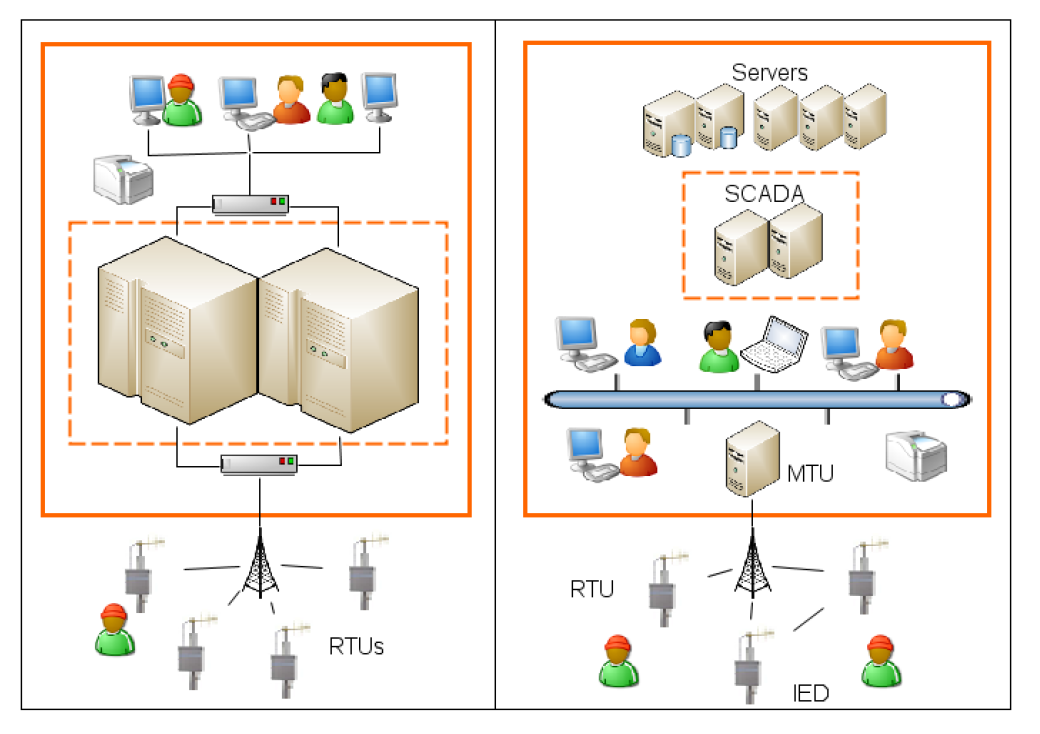
\includegraphics[width=\textwidth]{figures/SCADA-CentralisedAndDistributed.png}    


\caption[A Centralised and Distributed SCADA system]{A Centralised and Distributed SCADA system \cite[p. 123]{alcaraz2012security}}
\label{fig:SCADA-CentralisedAndDistributed}
\end{figure}



The characteristics of the three generations of SCADA systems described by \Citeauthor{alcaraz2012security} in \cite{alcaraz2012security}, may be summarised below:
 

 \begin{enumerate}
     \item A Monolithic SCADA system utilises a centralised offline control center  infrastructure, in order to monitor and control the physical system by proprietary control mechanisms.
     \item A Distributed SCADA system utilises a networked, but centralised control  center in order to monitor and control the physical system by proprietary control mechanisms. 
     \item A Networked SCADA system utilises a networked, and online control  center in order to monitor and control the physical system by standardised control mechanisms.
 \end{enumerate}



 \begin{figure}[ht]
\centering
    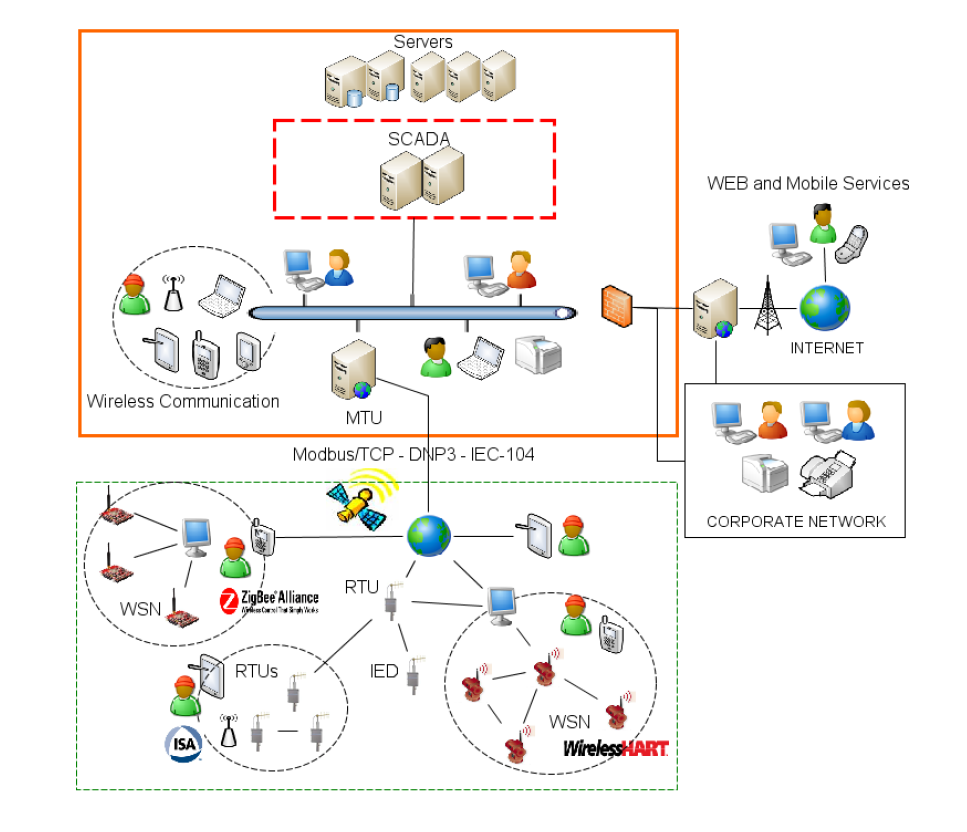
\includegraphics[trim=20 20 20 10, clip, width=\textwidth]{figures/SCADA-Current.png}
\caption[A Current SCADA system]{A Current SCADA system \cite[p. 124]{alcaraz2012security}}

\end{figure}





\subsection{The Modernised SCADA system}
 
 The \acrshort{scada} system is, as described in \cite{alcaraz2012security}, a system utilised to supervise and control \acrfull{ci} systems, including \acrshort{pg} infrastructures. Initially designed in order to control physical infrastructure systems like the classic \acrlong{pg}, the Monolithic SCADA system emerged into the Distributed SCADA system. The transition from a Monolithic SCADA system to a Distributed SCADA system transforms, as indicated by figure \ref{fig:SCADA-CentralisedAndDistributed}, the central management center from a centrally controlled mainframe environment, to a networked server environment controlled by operators connected through a \acrfull{lan}
  
  
 The \acrshort{sg} control center emerged from the Distributed SCADA system, into the Networked SCADA system used in order to control modern \acrlong{cps}s, like the \acrshort{sg}.\\ 
 


 





 




However, as explained by \Citeauthor{zamani2020introduction} in \Cite{zamani2020introduction}, the \acrshort{scada} system has a number of shortcomings, making it unsuitable for a \acrshort{sg} enegy distribution monitoring system:

\begin{itemize}
    \item The data polling rate is once every 2-10s, which is not sufficient in order to get real-time measurements.
    \item No time-stamps are attached to samples, making it hard to monitor rate of change over time
    \item State Estimation is not performed with sufficient frequency, if at all.
    \item The ability to observe dynamics is not supported by the system.
\end{itemize}





In order to address these shortcomings, the \acrfull{wams} system\footnote{WAMS is also known as the Wide Area \textbf{Monitoring} System}, described next, was invented.











\subsection{Wide Area Measurement System}
\begin{figure}[ht]
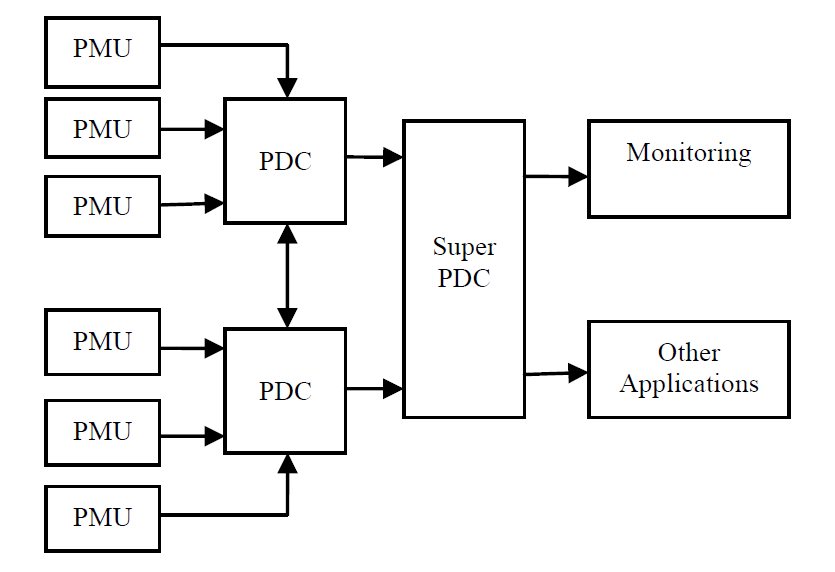
\includegraphics[width=\linewidth]{figures/Kumar-WAMS-architecture.png}
\caption[WAMS architecture]{WAMS architecture, as presented in \cite{kumar2015monitoring}}
\label{fig:Kumar-WAMS-architecture}
\end{figure}










\textit{DESCRIPTION:}
\textbf{\cite{kumar2015monitoring} \fullcite{kumar2015monitoring} }\\


    

In order to ensure the continuous monitoring of the modern \acrlong{sg} energy distribution system, the \acrfull{wams} is utilised. An overview of the \acrshort{wams} architecture, as presented in   \cite{kumar2015monitoring}, is shown as \figureautorefname  { } \ref{fig:Kumar-WAMS-architecture}:

The \acrshort{wams} is, as described in  \cite{kumar2015monitoring}, a  system, consisting of:

(1) \acrshort{pmu}s, (2) \acrshort{pdc}s, (3) The super \acrshort{pdc}, and (4) Communication networks.\\ 

The various components might be described as follows, from (4) to (1):
\begin{itemize}
    \item The \textbf{Communication Networks}, providing data transport between \acrshort{wams} components, as required.
    \item The \textbf{Super \acrshort{pdc}} controls several \acrshort{pdc}s constituting a distributed \acrshort{wams}.
\item The \textbf{\acrfull{pdc}} is responsible for collecting and interpreting \acrshort{pmu} measurements, before synchronising the measurements according to timestamps, in order to get more complete status information based on a combination of measurements.
    \item The \textbf{\acrfull{pmu}} is an intelligent measuring device, responsible for registering sensor measurements,  performing calculations like, for instance, phase angles, as well as voltage and current magnitudes. The data registered and processed by the \acrshort{pmu}, is transferred to the nearest \acrshort{pdc}.
    \end{itemize}

\begin{figure}[ht]
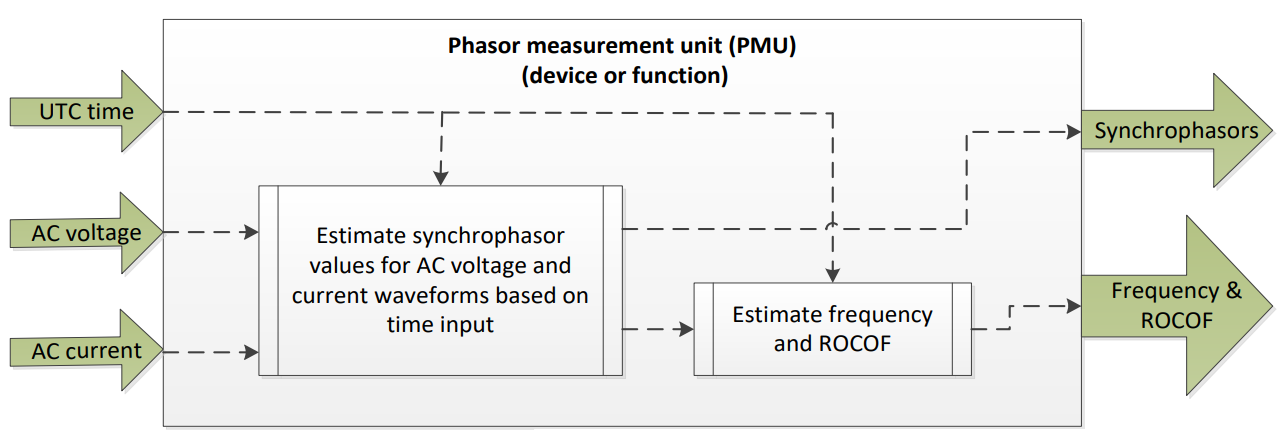
\includegraphics[width=\linewidth]{figures/PMU-in-out.png}
\caption[PMU inputs and outputs]{PMU inputs and outputs, as presented in \Cite[p.12]{iec2018measuring}
}
\label{fig:PMU-in-out}
\end{figure}


\subsection{Synchrophasor}
%\cite{ali2016wide}


%\Cite{rana2015exploring}

\begin{figure}[ht]
    \centering
    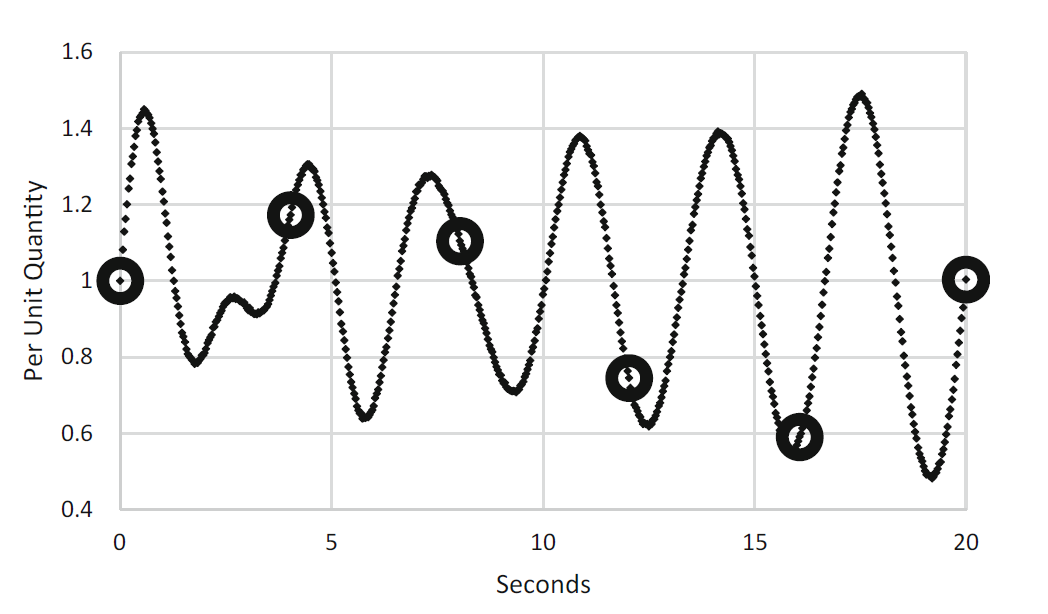
\includegraphics[ width=\textwidth]{figures/syncrophasors-vs-scada.png}
    \caption[Difference between Synchrophasor and SCADA measurements]{As presented in \cite[p. 3]{dagle2019importance}: Notional representation of the difference between synchrophasor and SCADA
measurement. Figure credit: \citeauthor{dagle2019importance}}.
    \label{fig:syncrophasors-vs-scada}
\end{figure}  



The \acrshort{pmu} is receiving values from sensors, on which it is able to calculate voltage level and phase angle of the energy flow. It is utilising a time-source to pinpoint measurements in time, producing synchrophasors, to be transmitted to the nearest \acrshort{pdc}. 

As described by \citeauthor{dagle2019importance} in \cite{dagle2019importance}, the data received from traditional \acrshort{scada} systems are time-stamped after arriving at the control station. The synchrophasors of the \acrshort{wams} on the other hand are, as described by \Citeauthor{ali2016wide} in \cite{ali2016wide}, being time-stamped in real-time before being transferred to the control system. The sampling rate of the \acrshort{pmu}, results in synchrophasor data enabling operators of the \acrshort{wams} to get real-time visualisation of critical elements, like the state of energy flow  of the \acrlong{sg}. The increased granularity of the measurement system allows for the detection of anomalies undetectable by traditional \acrshort{scada} systems, as illustrated by \figureautorefname { }\ref{fig:syncrophasors-vs-scada}. 

The increased sampling rate, of the synchrophasors of the \acrshort{wams} systems enables a more fine-grained view of energy distribution system state changes. However, in order for the \acrshort{wams} system to get the correct system state information, correct time stamps is critical. 
Therefore, the time-synchronisation mechanisms of the \acrshort{pmu} system is of critical importance. \\ 



The GPS signal transmits timing information, which enables 


$$t_{UTC}=t_{rcv}-t_{p}-\Delta t_{UTC}$$
A synchrophasor is, as described by 



%\textbf{TO DO:}
%\textit{Introduction:}

%\textit{What is it?}
%\textit{Which functions does it have?}





%Explain TimeSync 





A periodic signal $x(t)=X_m\cos\left(\omega t+\phi \right)$ has, according to \Cite{schofield2018design}, a synchrophasor representation $\mathbf{X}$, defined by $ \mathbf{X} = \frac{X_m}{\sqrt{2}}e^{j\phi} $ where $ \mathbf{X} = |X| = X_m / \sqrt{2} $ is  the RMS and $  \phi = angle(\mathbf{X}) $ is the angle.


%\[x(t)=X_m\cdot\cos\left(\phi + \int\displaylimits_{-\infty}^t\omega (\tau)\cdot\mathrm{d}\tau\right)\]

%\[\overline{X} = X_m{\angle\phi} \]


\begin{figure}[t]
    \centering
    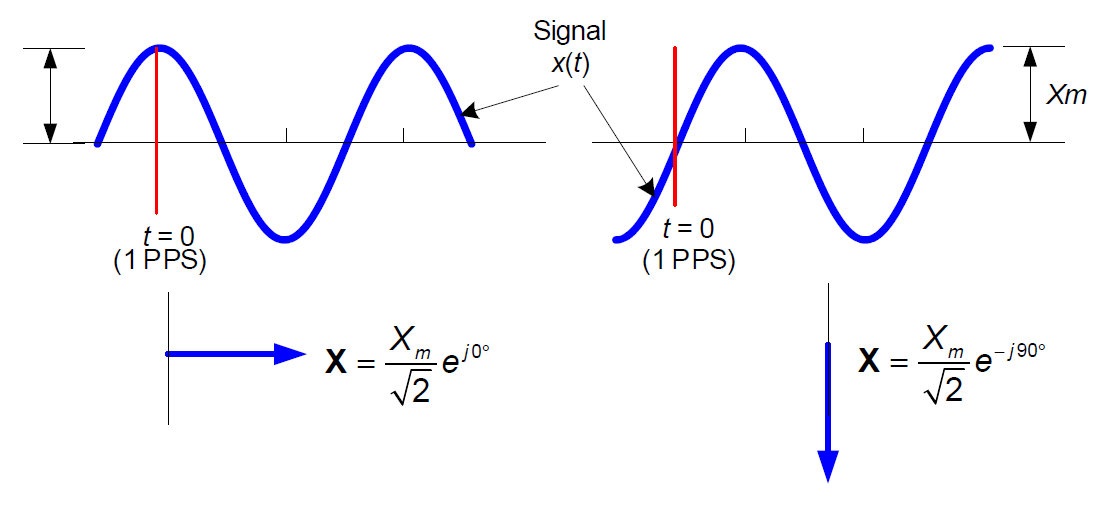
\includegraphics[ width=\textwidth]{figures/Synchrophasor-Definition.png}
    \caption[Convention for synchrophasor representation]{As presented in \Cite{schofield2018design}: Convention for synchrophasor representation.}.
    \label{fig:Synchrophasor-Definition}
\end{figure}  



\section{Time Synchronisation}
In order to synchronise the samples received from the \acrshort{pmu}, the \acrshort{pdc}, as well as the \acrshort{pmu} devices producing the samples, is required to adjust their clock by utilising a precise and reliable times source.  Given the distributed nature of the \acrshort{pmu} devices providing samples from locations distributed over a Wide Area Network, the \acrfull{gps} is the  time source selected. 

\subsection{Introduction}


The dependency on networking favors the usage of low-cost \acrshort{gnss} receivers for synchronising time between the growing number of \acrshort{pmu}s deployed at various locations, monitoring energy flow states of the highly distributed \acrshort{sg}. 



\subsection{The Importance of Time Synchronisation}

In \cite{dagle2019importance}, \citeauthor{dagle2019importance} states the following aspects as the benefits for Smart Grid operation, of ensuring correct time synchronisation:


\begin{itemize}
    \item  Situational Awareness and Wide-Area Monitoring
    \item  Real-Time Operations
    \item  Power System Planning 
    \item  Forensic Event Analysis
    
\end{itemize}

\subsection{Possible effects of Time Synchronisation errors}
Timing errors will, according to ,,, render the data introduced to the \acrshort{wams} system inadequate to enable \acrshort{sg} operatiors to get overview of the Energy supply state of the \acrshort{sg}.

In \Cite{martin2019impact}, \citeauthor{martin2019impact} lists a number of side-effects which could result form the absence of high-quality data material from the \acrshort{wams}.


\begin{enumerate}




    \item Data loss,
    \item Data corruption,
    \item Inaccurate representation of engineering quantities,
    \item Lack of precision,
    \item Incorrect measurement identification,
    \item Excessive or inconsistent latency.

\end{enumerate}

\subsection{Smart Grid Time Synchronisation}


\subsubsection{Introduction}


The \acrlong{sg} is dependant on precise Time Synchronisation, as a Time Synchronisation error of a few $\mu$-seconds may result in \acrshort{sg} instability. The time stamps produced by Synchrophasors, pinpointing the exact time of any system event, is vital in order to ensure precise and reliable system state information.
In the event of a system alert being triggered by erroneous system state Information, corrective actions by operators might have undesired effects. 

\subsubsection[Smart Grid Time Sync Precision Requirements]{Smart Grid Time Synchronisation Precision Requirements}

In order to ensure the time precision required for the \acrshort{sg}, the correct selection of time synchronisation mechanisms is vital. 
\section{Time Synchronisation Sources}

As described by \citeauthor{moussa2016security} in \cite{moussa2016security}, both PTP and GNSS is able to achieve the precision level required, as opposed to NTP and PPS.  Based on this observation, the \acrshort{tsa} Detection and Mitigation coverage is limited to \acrshort{gnss} and  \acrshort{ptp} systems only.




\subsection{Global Navigation Satellite Systems}

A \acrfull{gnss}, is a system of communication satellites orbiting the Earth, in order to determine the current position for, usually,\footnote{\acrlong{sg} systems utilises \acrshort{gnss} systems for time synchronisation, not navigational, purposes.} navigation  purposes. As described by \citeauthor{schmidt2016survey} in \cite{schmidt2016survey}, there exists several \acrshort{gnss} constellations,\footnote{In \cite{schmidt2016survey}, both the United States "GPS" and the Russian "GLONASS" systems, as well as the European "Galileo" and the Chinese "Beidou-2" systems are mentioned.} each being classified as "strikingly similar" to the other \acrshort{gnss} systems. 



%Therefore, any description of \acrshort{gnss} systems, as well as attacks targeting them, will be considering the well-known \acrfull{gps} system only.





As described by \citeauthor{schmidt2016survey} in  \cite{schmidt2016survey},  a \acrshort{gnss} system transmits three different messages:

\begin{enumerate}
    \item A PVT ranging signal for Position, Velocity, and Timing.
    \item Precise Ephemeris\footnote{Ephemeris is calculated based on prior observations of astronomical object trajectories} data, is specifying the exact location of each satellite.
    \item An almanac used in order to select satellites for tracking, based on the known location of all satellites. 
    
\end{enumerate}

$$r(t)=\sum_{k=1}^{32}H_{k}(2P_{c})^{\frac{1}{2}}(C_{k}(t)\oplus D_{k}(t))\cos{2\pi}(f_{L1}+\Delta f_{k})t+n(t) $$


As further described by \citeauthor{schmidt2016survey}, satellites from any other \acrshort{gnss} constellation may be used in order to avoid problems related to poor reception or blackout which would, possibly be the result of using same constellation satellites only.


The \acrshort{gnss} signal is utilised in order to provide time synchronisation between \acrshort{sg} \acrshort{pmu} devices, in order to enable the \acrshort{wams} system operators to get the best available 
view of \acrshort{sg} distribution system state.


\subsubsection{Description of GSSN time synchronisation}
The time signal available from \acrfull{gnss} systems is by several papers described as the major contributor to the wide-spread usage of \acrshort{pmu}s in order to monitor \acrlong{sg} energy flow status. 





\subsection{Precision Time Protocol services}
The \acrfull{ptp} is a network-based time protocol, enabling the time difference between devices to be synchronised within a fraction (in the order of a few $\mu$s) of a second, satisfying the requirements of the \acrshort{sg}. 

\begin{figure}[ht]
    \centering
    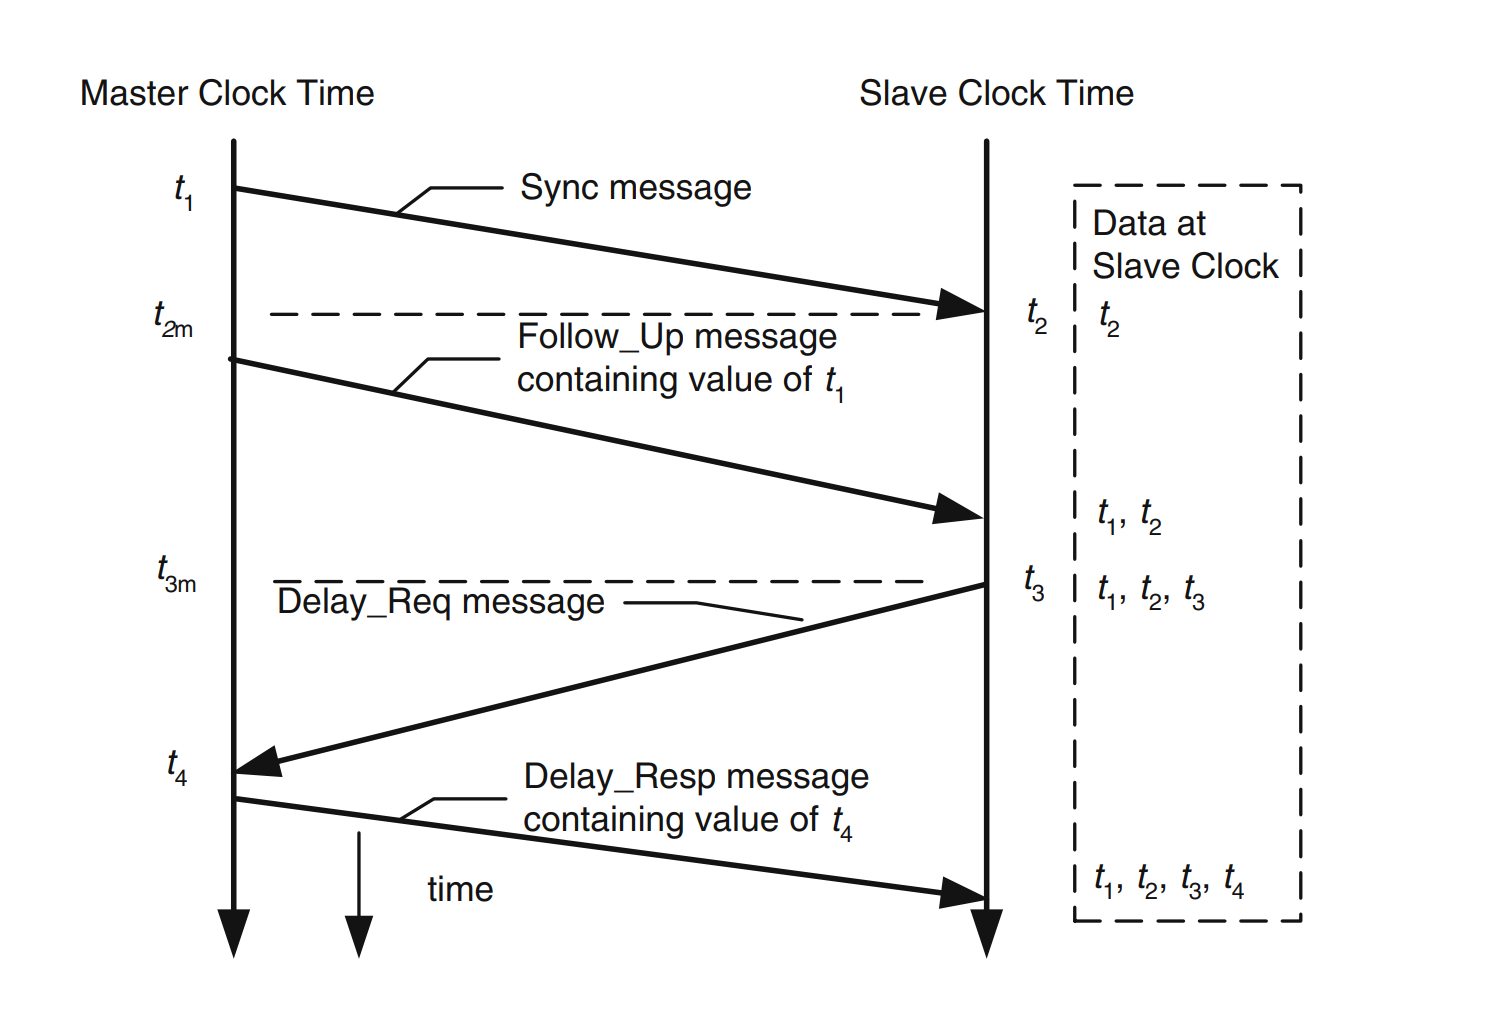
\includegraphics[ width=\textwidth]{figures/PTP-timing-Diagram.png}
    \caption[Timing diagram for synchronization messages]{As presented in \cite[p. 51]{Eidson2006}: Timing diagram for synchronization messages.} 
    \label{fig:PTP-timing-Diagram}
\end{figure}  

\subsubsection{Description of PTP time synchronisation}



A device, being synchronised  by the \acrshort{ptp} protocol, reads its system time from a slave clock, being periodically synchronised with a master clock.


The time of the slave clock, is being adjusted according to the following process:


Following the message exchange visualised by \figureautorefname { } \ref{fig:PTP-timing-Diagram}, the Slave clock  uses the time offset from the Master clock time, $offset = [(t_2 - t_1) + (t_4 - t_3)]\div 2$, in order to synchronise with the Master clock. \\ 

In order to be able to achieve the time difference required, the \acrshort{ptp}, as described by  \citeauthor{Eidson2006}, in \cite{Eidson2006}, is dependant on:

\begin{itemize}
    \item Timestamped network events, messages, which is  used for synchronisation.
    \item A method of timestamp transmission as required for synchronisation.
    \item Overcoming any timing impairments introduced by system components.
\end{itemize}

\section{Smart Grid Network Reliability and Security}

Two interrelated concepts are essential for the safe operation of the \acrshort{sg}:  
\begin{itemize}
    \item \acrlong{sg} \textbf{Network Reliability } which is important for the correct \acrshort{sg} operation, minimising the risk of \acrshort{sg} operational failures caused by \textbf{unintentional disruptive events} affecting \acrshort{sg} operations.
    
    \item \acrlong{sg} \textbf{Network Security}  which is important for the correct \acrshort{sg} operation, minimising the risk of \acrshort{sg} operational failures caused by \textbf{intentional malicious events}  affecting \acrshort{sg} operations.
\end{itemize}



\subsection{Smart Grid Network Reliability}

\subsection{Smart Grid Network Security}


    
\section{Cyber Attacks}



Computer systems reachable\footnote{Systems could ultimately be targeted utilising USB sticks, if not accessible from the Internet.} from the outside world,  are potential targets of Cyber attacks. The eventual recoveries of the initial Cyber Attacks was followed up by defence actions, resulting in more advanced attack techniques, has evolved to a continuous battle of control between attackers and defenders. \\


There are numerous Threat Actors of various skill levels, from so-called "Script Kiddies" to professionals, aiming to get unauthorised access to systems, for fun, fame, or for more serious reasons, like terrorism or financial gain. 





\subsection{Cyber Attack models}

In order to analyse previous attacks, as well as to avoid future attacks, models have been developed. 

\Cite{straub2020modeling}

%\subsubsection{The Diamond model}
 \subsubsection{MITRE ATT\&K framework}
 
 
 \Cite{strom2018mitre}
\subsubsection{STRIDE}

\cite{khan2017stride}


\subsubsection{The Cyber kill chain}
The Cyber Kill Chain is a model designed for the analysis of attacks on Information Technology infrastructure. The model is an adoption of the military kill chain model developed by armed forces, based on prior military experience.
\begin{enumerate}
    \item \textbf{Reconnaissance} Information gathering on the target, utilising publicly available resources.
    \item \textbf{Weaponization} Preparation of malicious payload off target premises.
    \item \textbf{Delivery} Intruding the premises of the target, with malicious intents.  
    \item \textbf{Exploitation} Any activity related to information gathering on th premises of the target.
    \item \textbf{Installation} of any malicious software relevant for the attack
    \item \textbf{Command and control} A means by which the attacker establishes a control channel, enabling further actions.
    \item \textbf{Action on objectives} relative to the intents of the attack: Stealing information, controlling equipment, causing service disruption or termination.
\end{enumerate}
Given the complexity of \acrlong{ics}s, consisting of internal security barriers protecting critical system elements, it has not proven to be optimal for analysing attacks on the \acrshort{sg}.\\ 

Following the introduction of the Cyber Kill Chain, the model has been extended to be more suitable for the analysis of more specialised systems, like the \acrshort{sg}.
For the purpose of this thesis, the \acrfull{ics} Cyber Kill Chain, is described.
\subsubsection{The ICS Cyber kill chain}



\subsection{Time Protocol Threats}
Given the criticality of Time Synchronisation for the correct operation of the \acrshort{sg}, it is of vital importance to be aware of which threats imposes security risks related to the underlying Time Protocol. As explained by \citeauthor{mizrahi2014security} in \Cite{mizrahi2014security}, several attacker types could inflict a number of attacks on various time protocols. My introductory coverage of time protocol threats includes descriptions on attacker types and attack types, for reference purposes.

\subsubsection{Attacker Types}

\begin{itemize}
    \item The \textbf{Internal attacker} has privileged access to, at least parts of, the internal infrastructure of the target, enabling the ability to take malicious actions not available to non-internal attackers.
    \item The \textbf{External attacker} is limited to attacking the targeted infrastructure from the outside, typically through network connections.
    \item The \textbf{Traffic Injector attacker} adds network packages to the benign traffic of the networks of the target, in order to produce the desired effects on the state and operation of the targeted infrastructure. 
    \item The \textbf{\acrshort{mitm} attacker} interrupts the communication between the two parties A and B, impersonating as B to A and vice-versa.
\end{itemize}



The various types of attackers possesses various malicious action capabilities, which they may use in order to attack their intended target in numerous ways.


\subsubsection{Attack Types}
As described in \cite{mizrahi2014security}, a number of threats affecting the \acrshort{ntp} and  \acrshort{ptp} time protocols is observed:



\begin{itemize}
    \item Grand Master Time Source Attack
    \item \acrfull{dos} attacks: Specialised protocol-specific \acrshort{dos} attacks, as well as traditional IP-based \acrshort{dos} attacks.
    \item Cryptographic Performance Attacks
    \item Packet Manipulation Attacks
    \item Spoofing Attacks
    \item Replay Attack   
    \item Rouge Master attack 
\end{itemize}






\subsection{Advanced Persistent Threat (APT)}

The most advanced, sometimes stealthy, Cyber Attacks are imposing an imminent uncertainty amongst those tasked with the safe operation of critical systems like the \acrshort{sg}. Threat Actors capable of breaking in to presumably secure critical systems, staying undetected for several months or years, constitutes a persistent threat to the secure operation of the system.


